\documentclass[e4_tp3_main.tex]{subfiles}
\begin{document}
\newgeometry{top=2.5cm, bottom=2.0cm, left=2.25cm, right=2.25cm}

\section{Control de velocidad de motores de inducción trifásicos}
Se procedió a analizar el circuito con el cual se realiza un control sobre un motor trifásico.
\subsection{Análisis a lazo abierto}
En esta etapa, vamos a realizar un análisis sobre el circuito a lazo abierto. Para ello, se dispuso del circuito de la siguiente forma:
\begin{figure}[H]
\centering
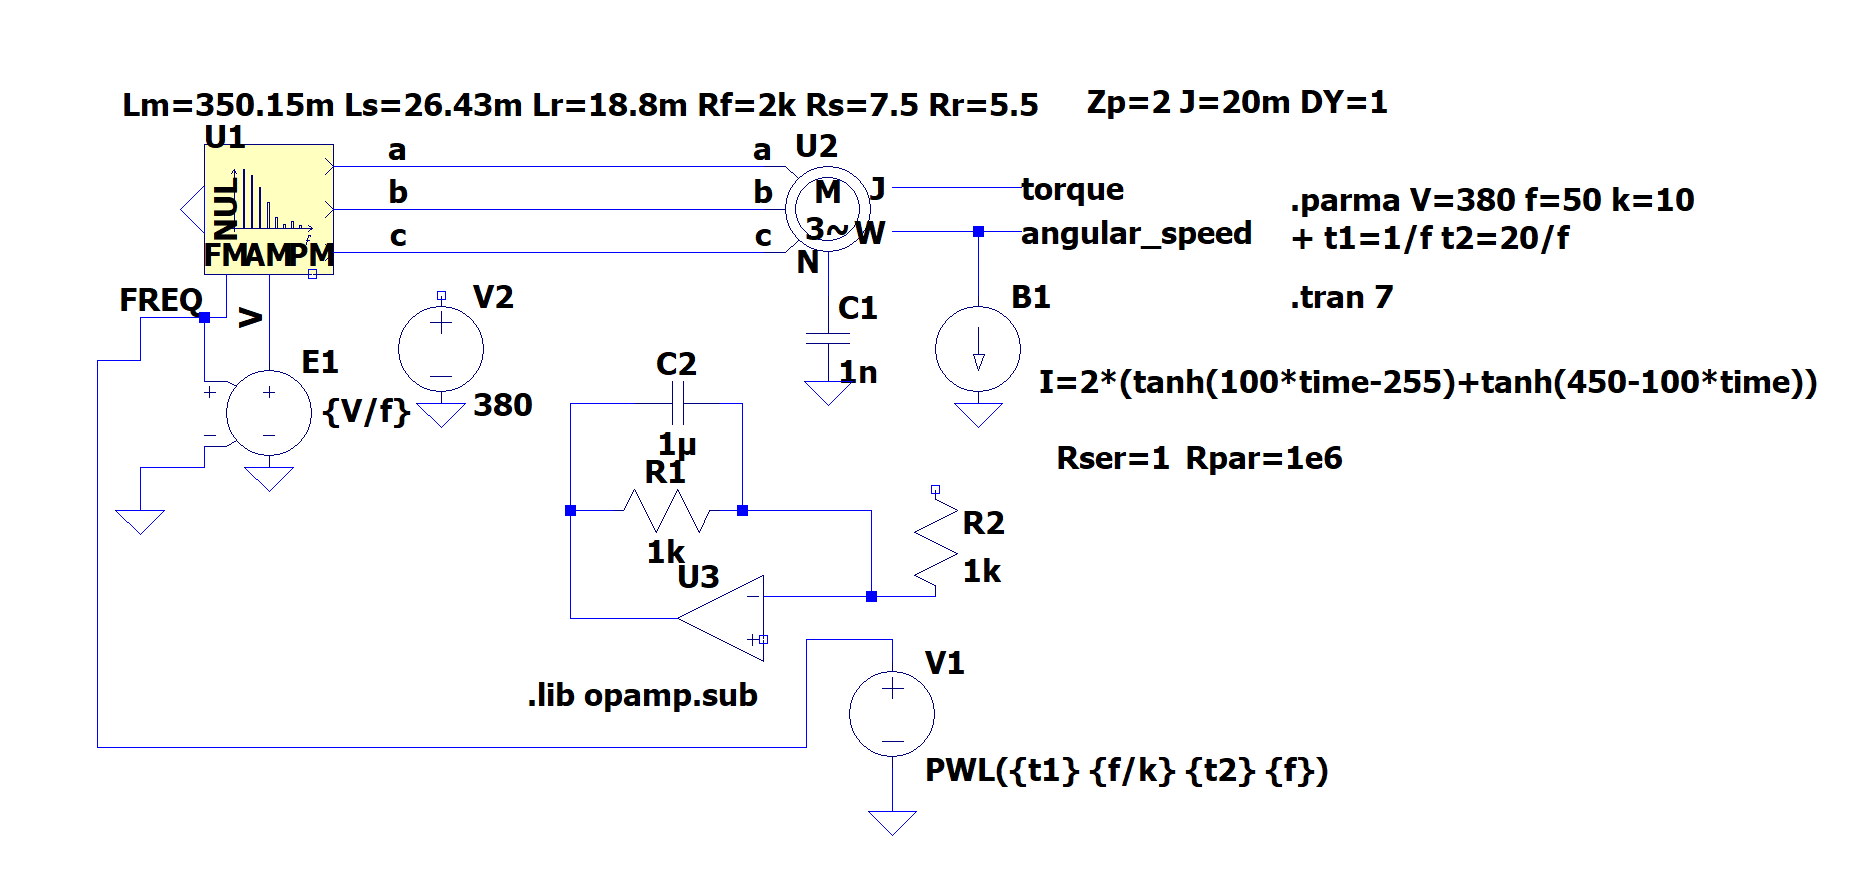
\includegraphics[width=0.5\linewidth]{Imagenes/3-1-a-circuito.png}
\caption{Diagrama del circuito a lazo abierto}
\end{figure}

Una vez configurado el generador con N=2k+1 a fin de insertar armónicos en la tensión de línea, obtuvimos los siguientes resultados:
\begin{figure}[H]
\centering
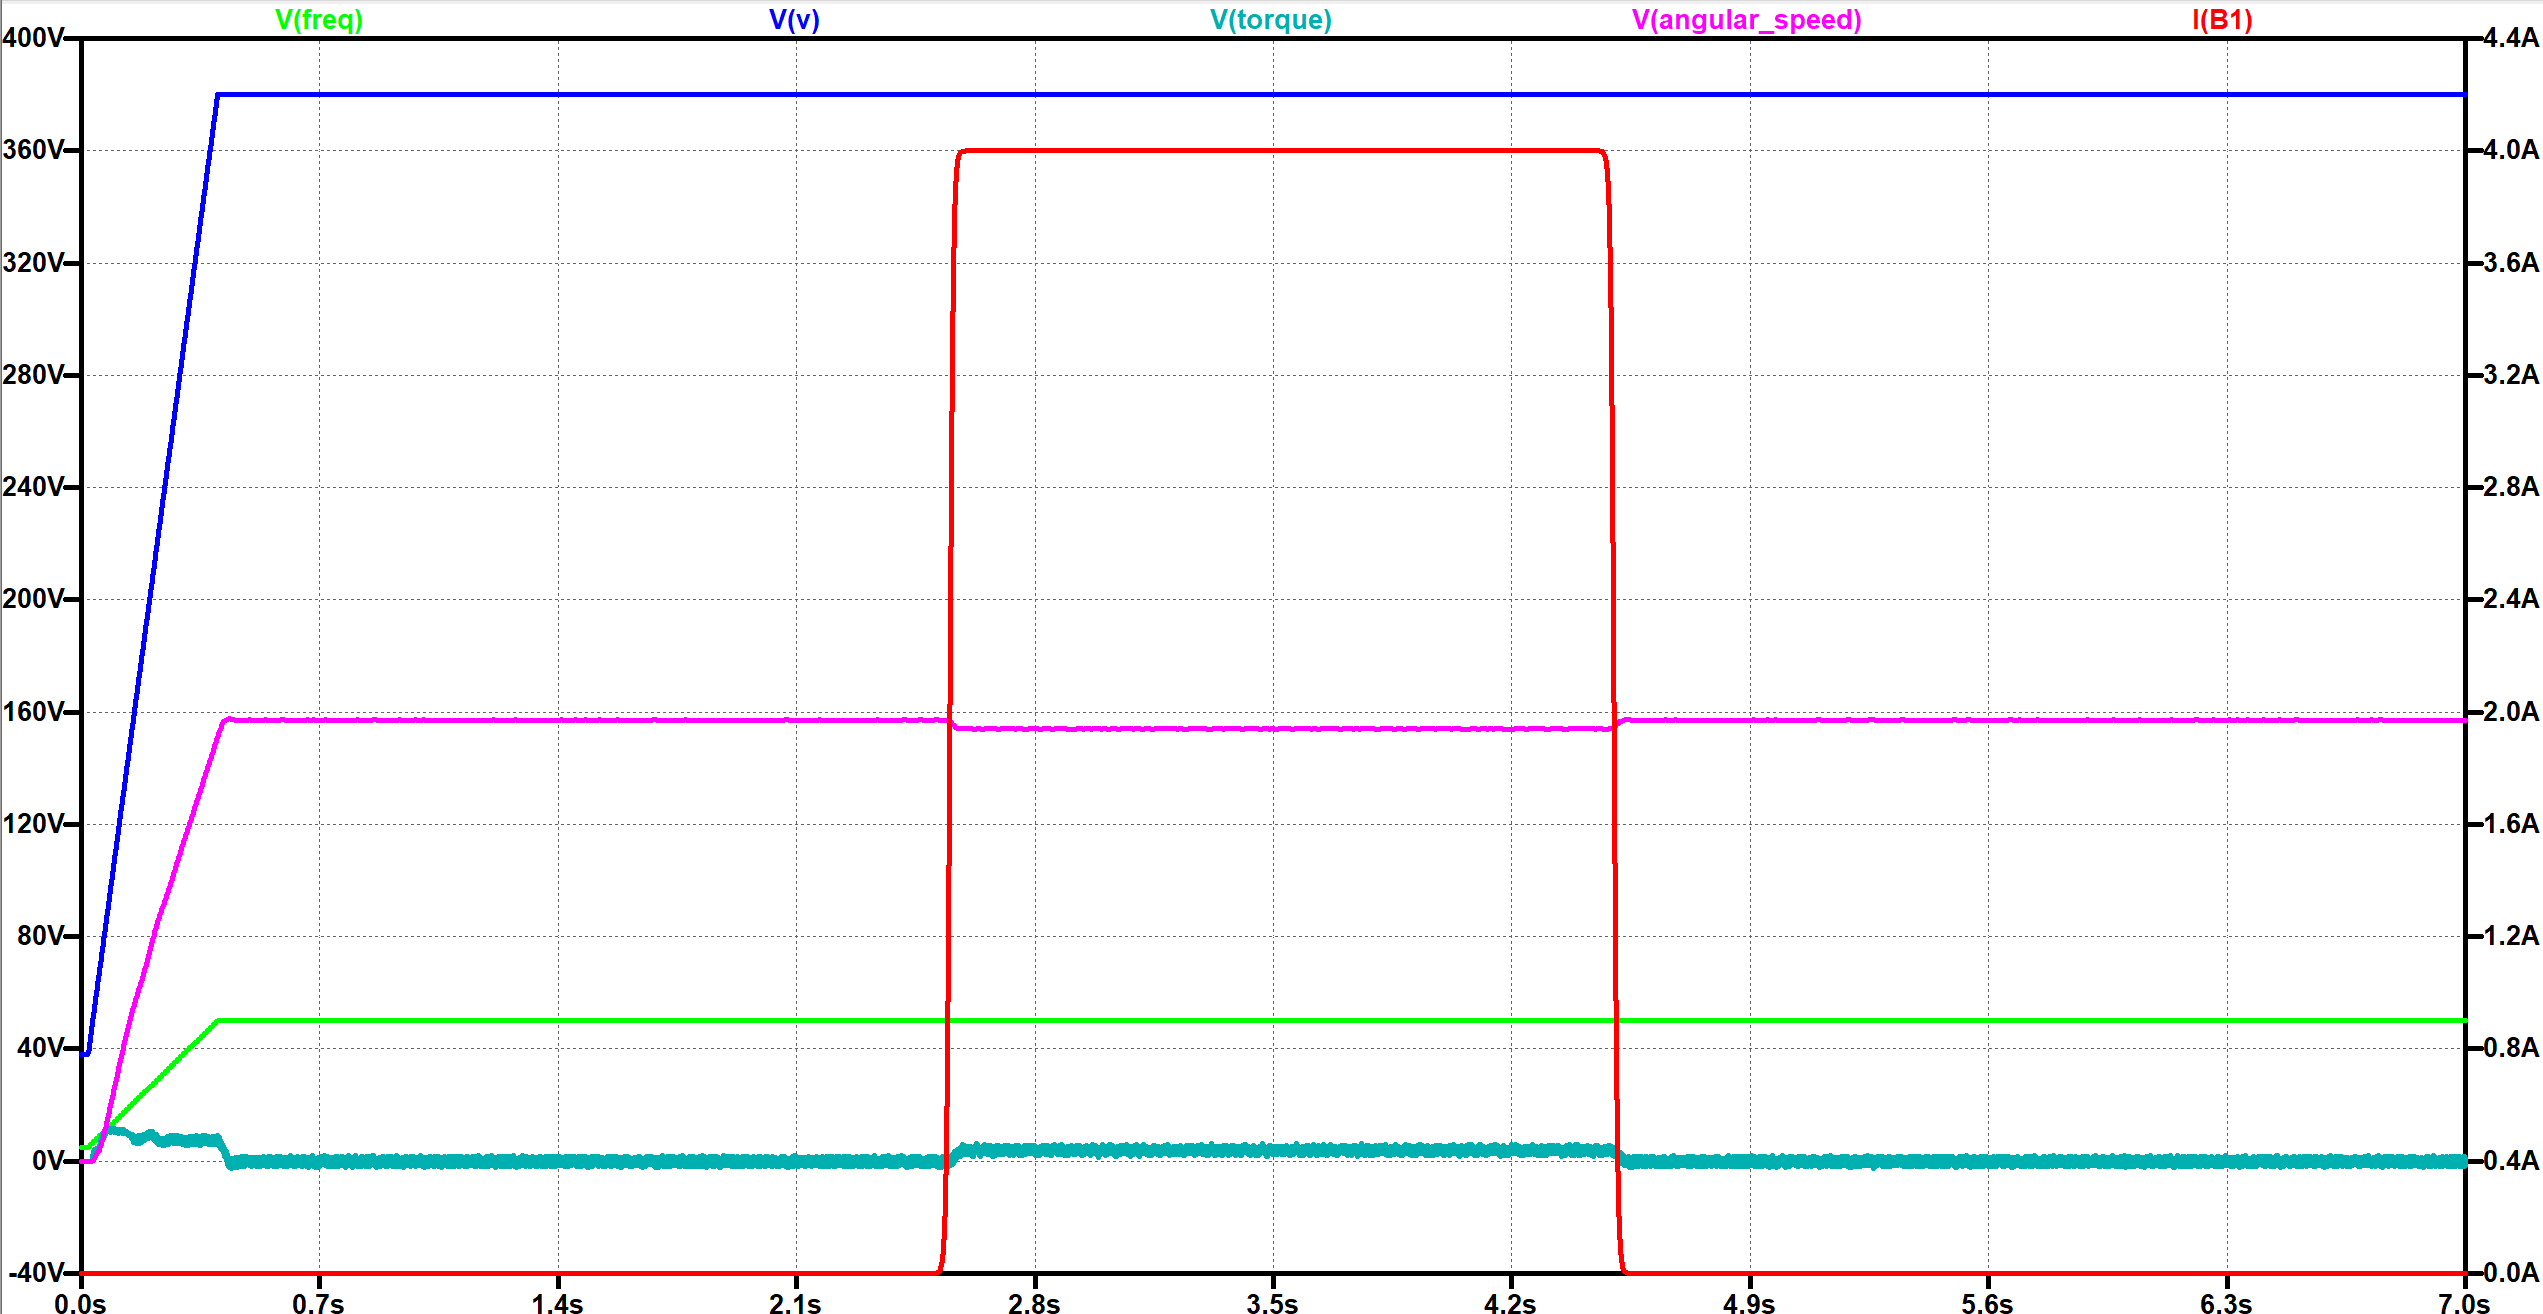
\includegraphics[width=0.75\linewidth]{Imagenes/3-1-a-general.png}
\caption{Diagrama temporal de la simulación del circuito}
\end{figure}

En la figura podemos observar cómo se comportan las señales de frecuencia del motor (representada por la tensión $V(FREQ)$), su velocidad angular (representada por la tensión $V(angular\_speed)$), el torque(representado por la tensión $V(torque)$), la carga (representada por la corriente $I(B)$) y la tensión de línea (representada por la tensión $V(V)$).
\begin{figure}[H]
\centering
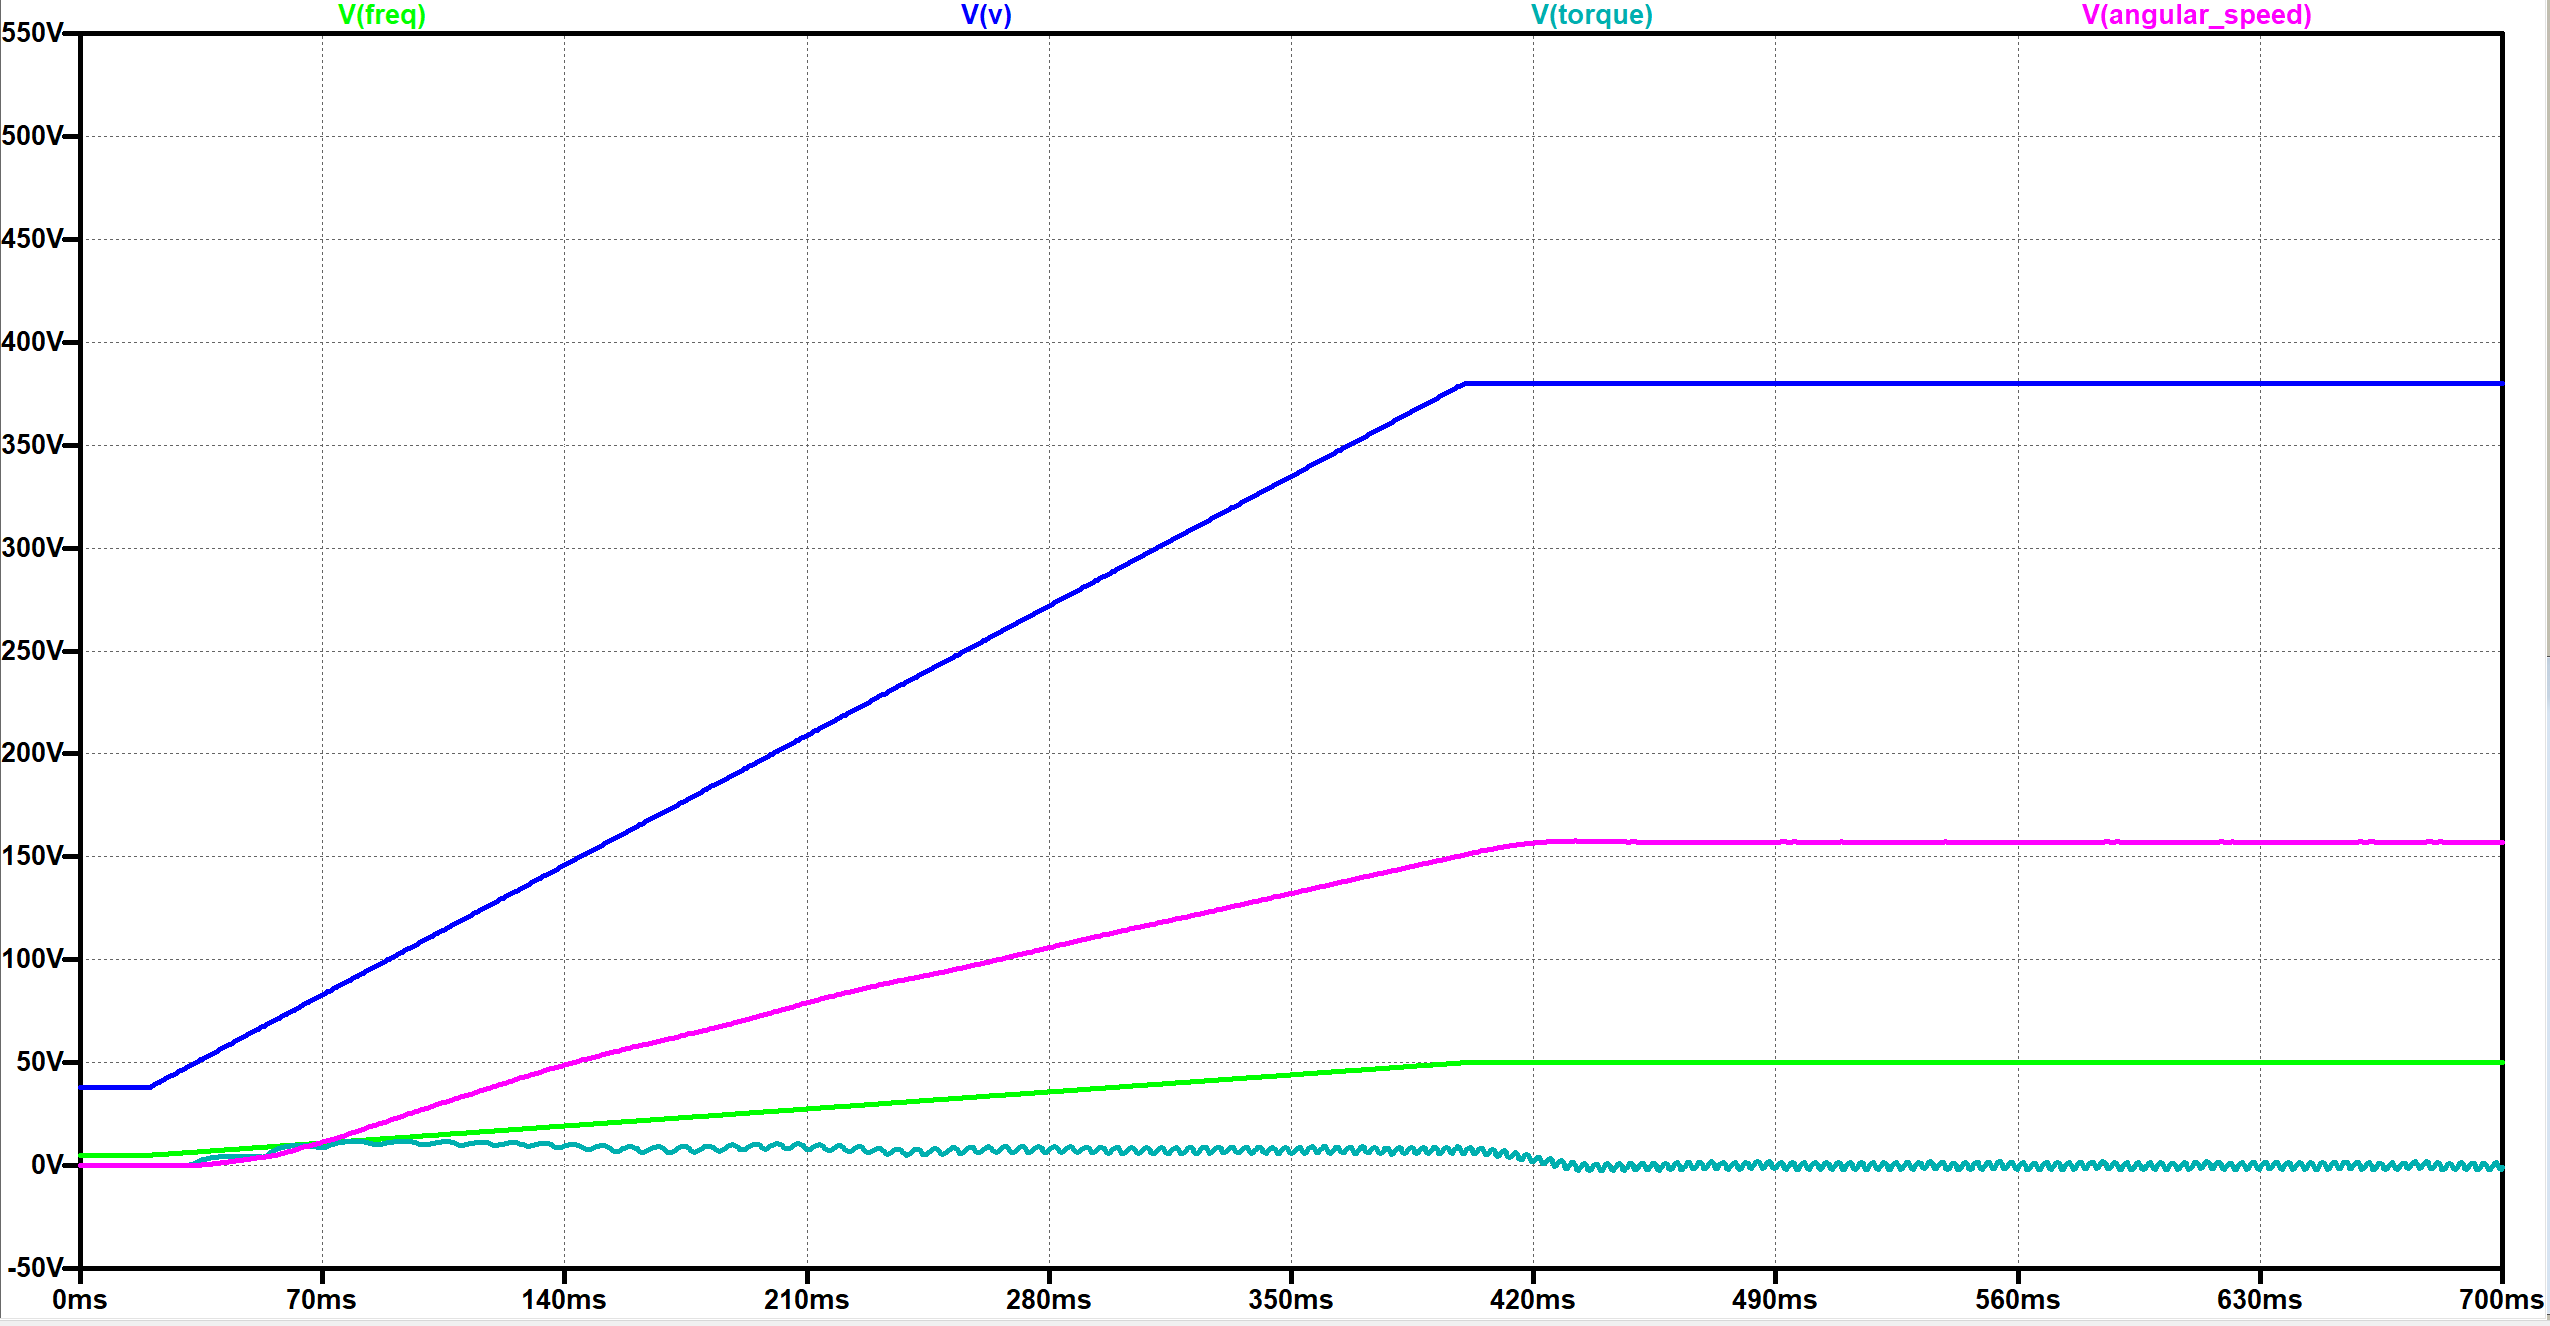
\includegraphics[width=0.7\linewidth]{Imagenes/3-1-a-inicio.png}
\caption{Diagrama temporal del encendido del circuito}
\end{figure}

Ni bien se enciende el circuito, observamos como la tensión de la línea sube de forma lineal desde 0 a 380V, y de igual manera,suben la frecuencia y la velocidad angular. Cuando aparece el primer $\Delta V_l$ lo que ocurre es que ,gracias a que mantengo el factor $\frac{V}{f}=cte$,el torque sube inmediatamente a su valor máximo, y se mantiene en ese valor hasta que el motor alcanza su velocidad máxima. Cuando el motor alcanza su $\omega_{max}$ el torque disminuye a 0. Observamos que en ese instante, la tensión de línea ya se encuentra en los 380V deseados, y la frecuencia se encuentra constante en 50 V (medidos).

Una vez que tenemos el motor girando a máxima velocidad, mediante el drenaje de una corriente I(B) lo que hacemos es simular una carga que se le coloca al motor. Al aplicar dicha corriente observamos lo siguiente:
\begin{figure}[H]
\centering
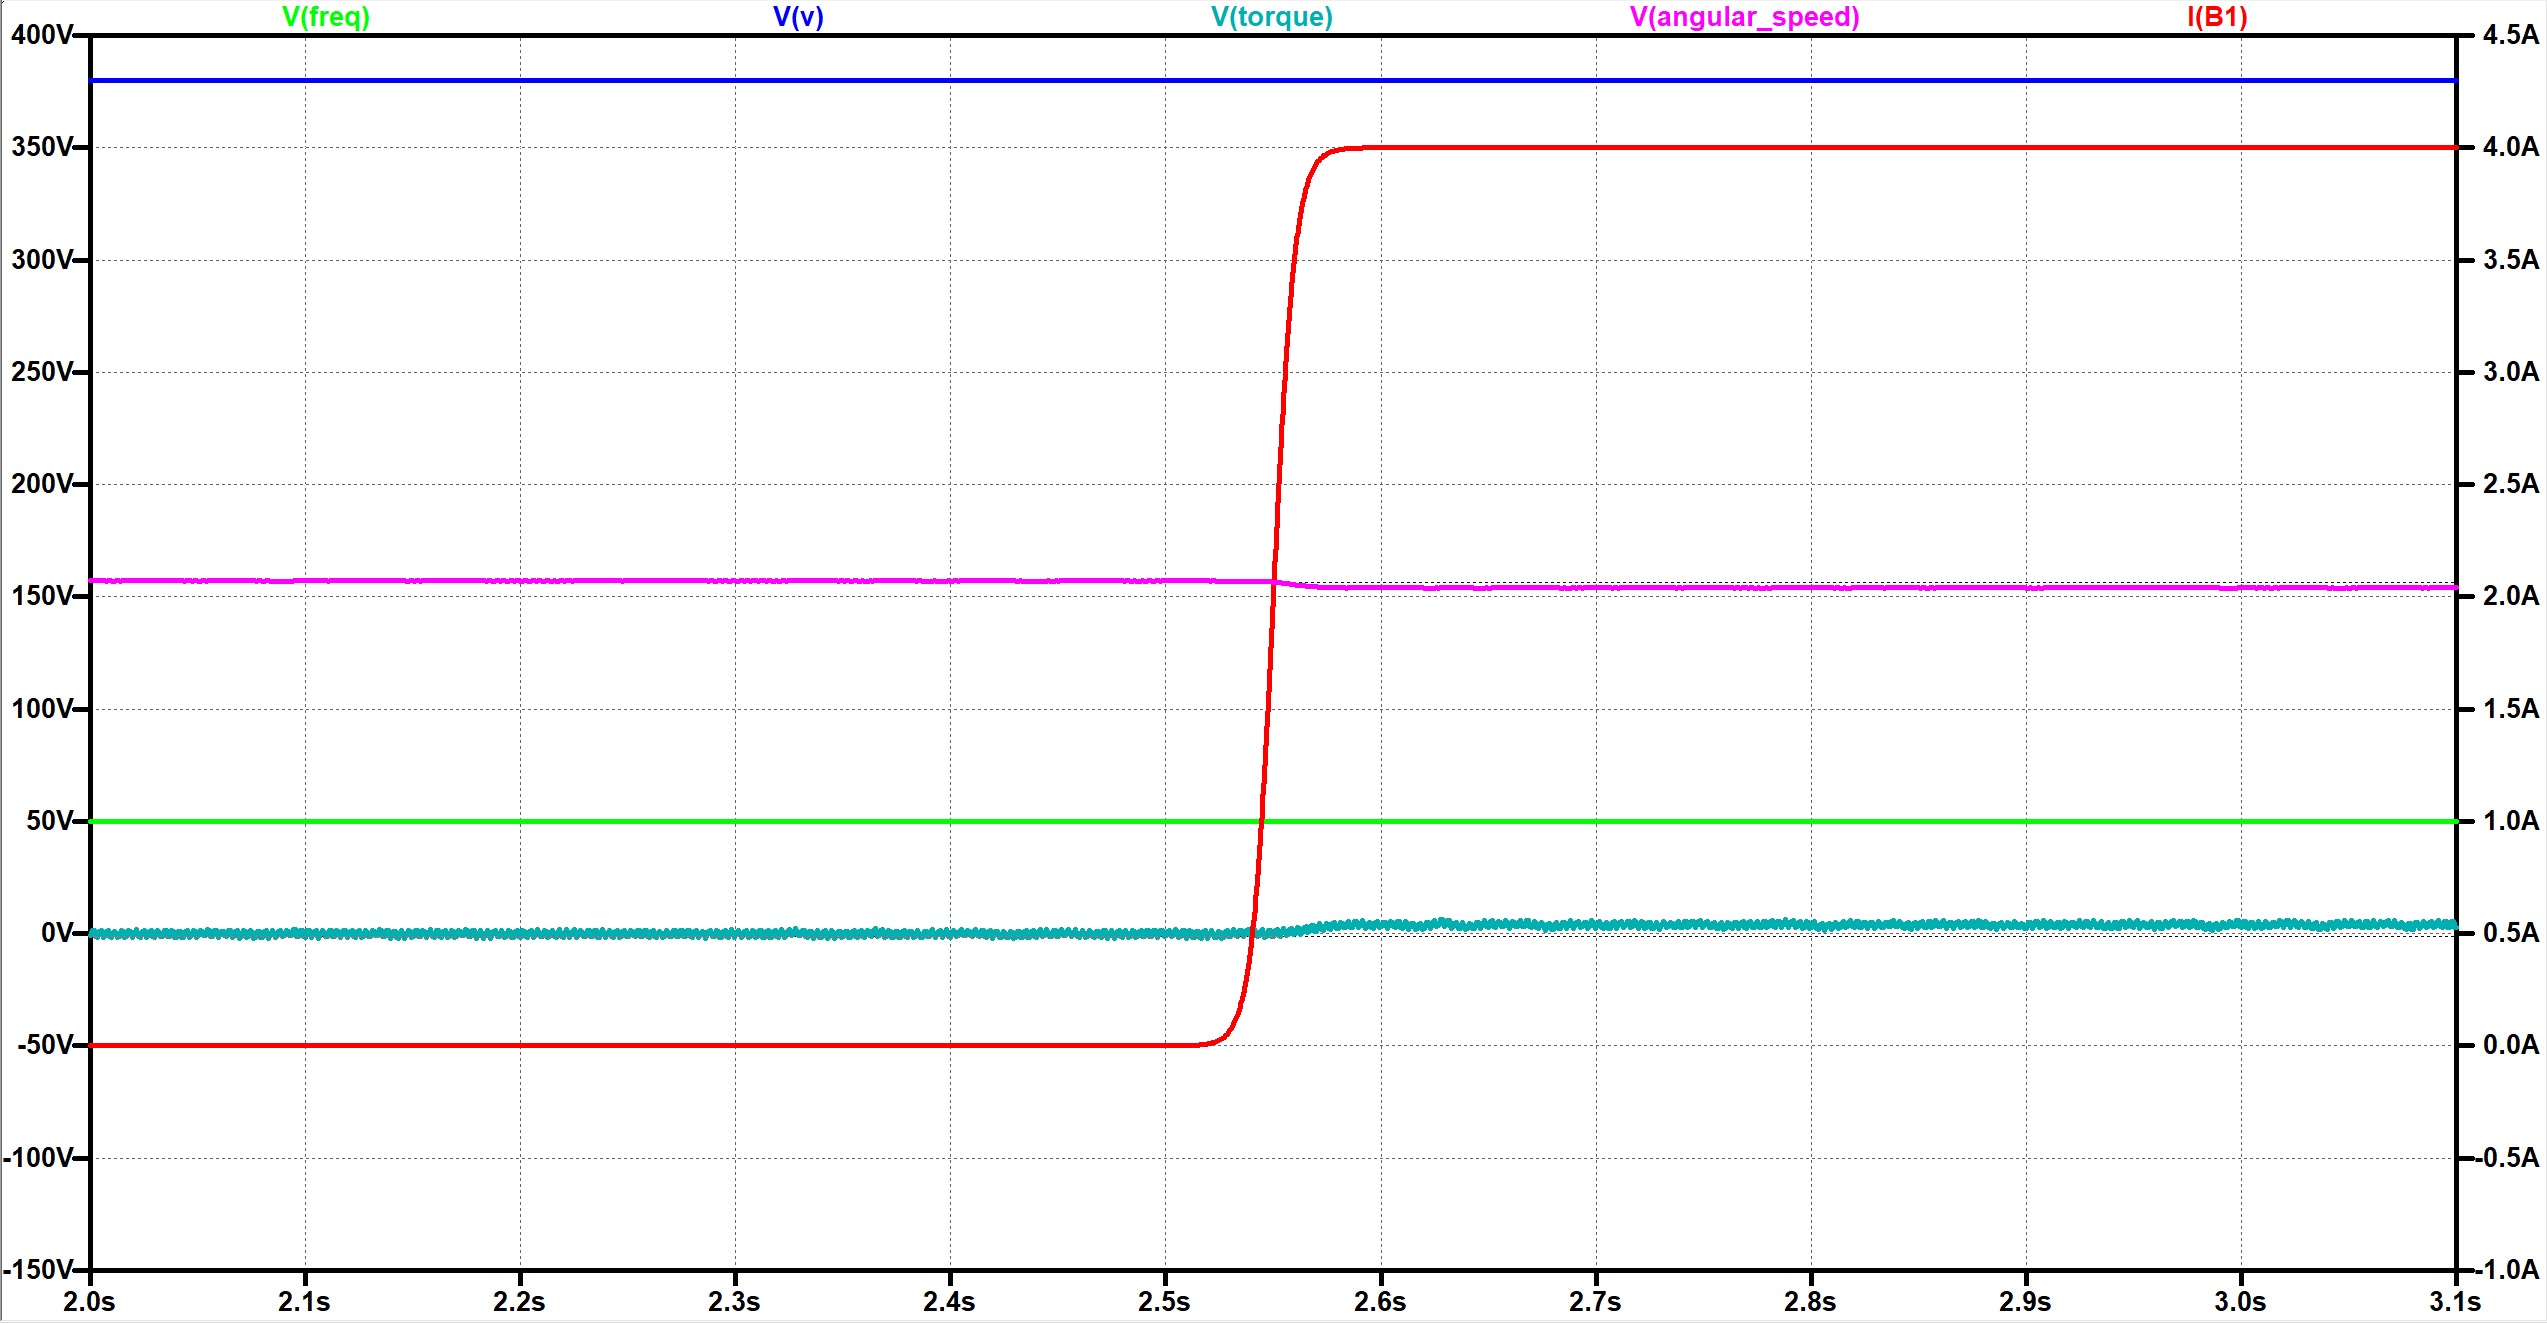
\includegraphics[width=0.45\linewidth]{Imagenes/3-1-a-carga.png}
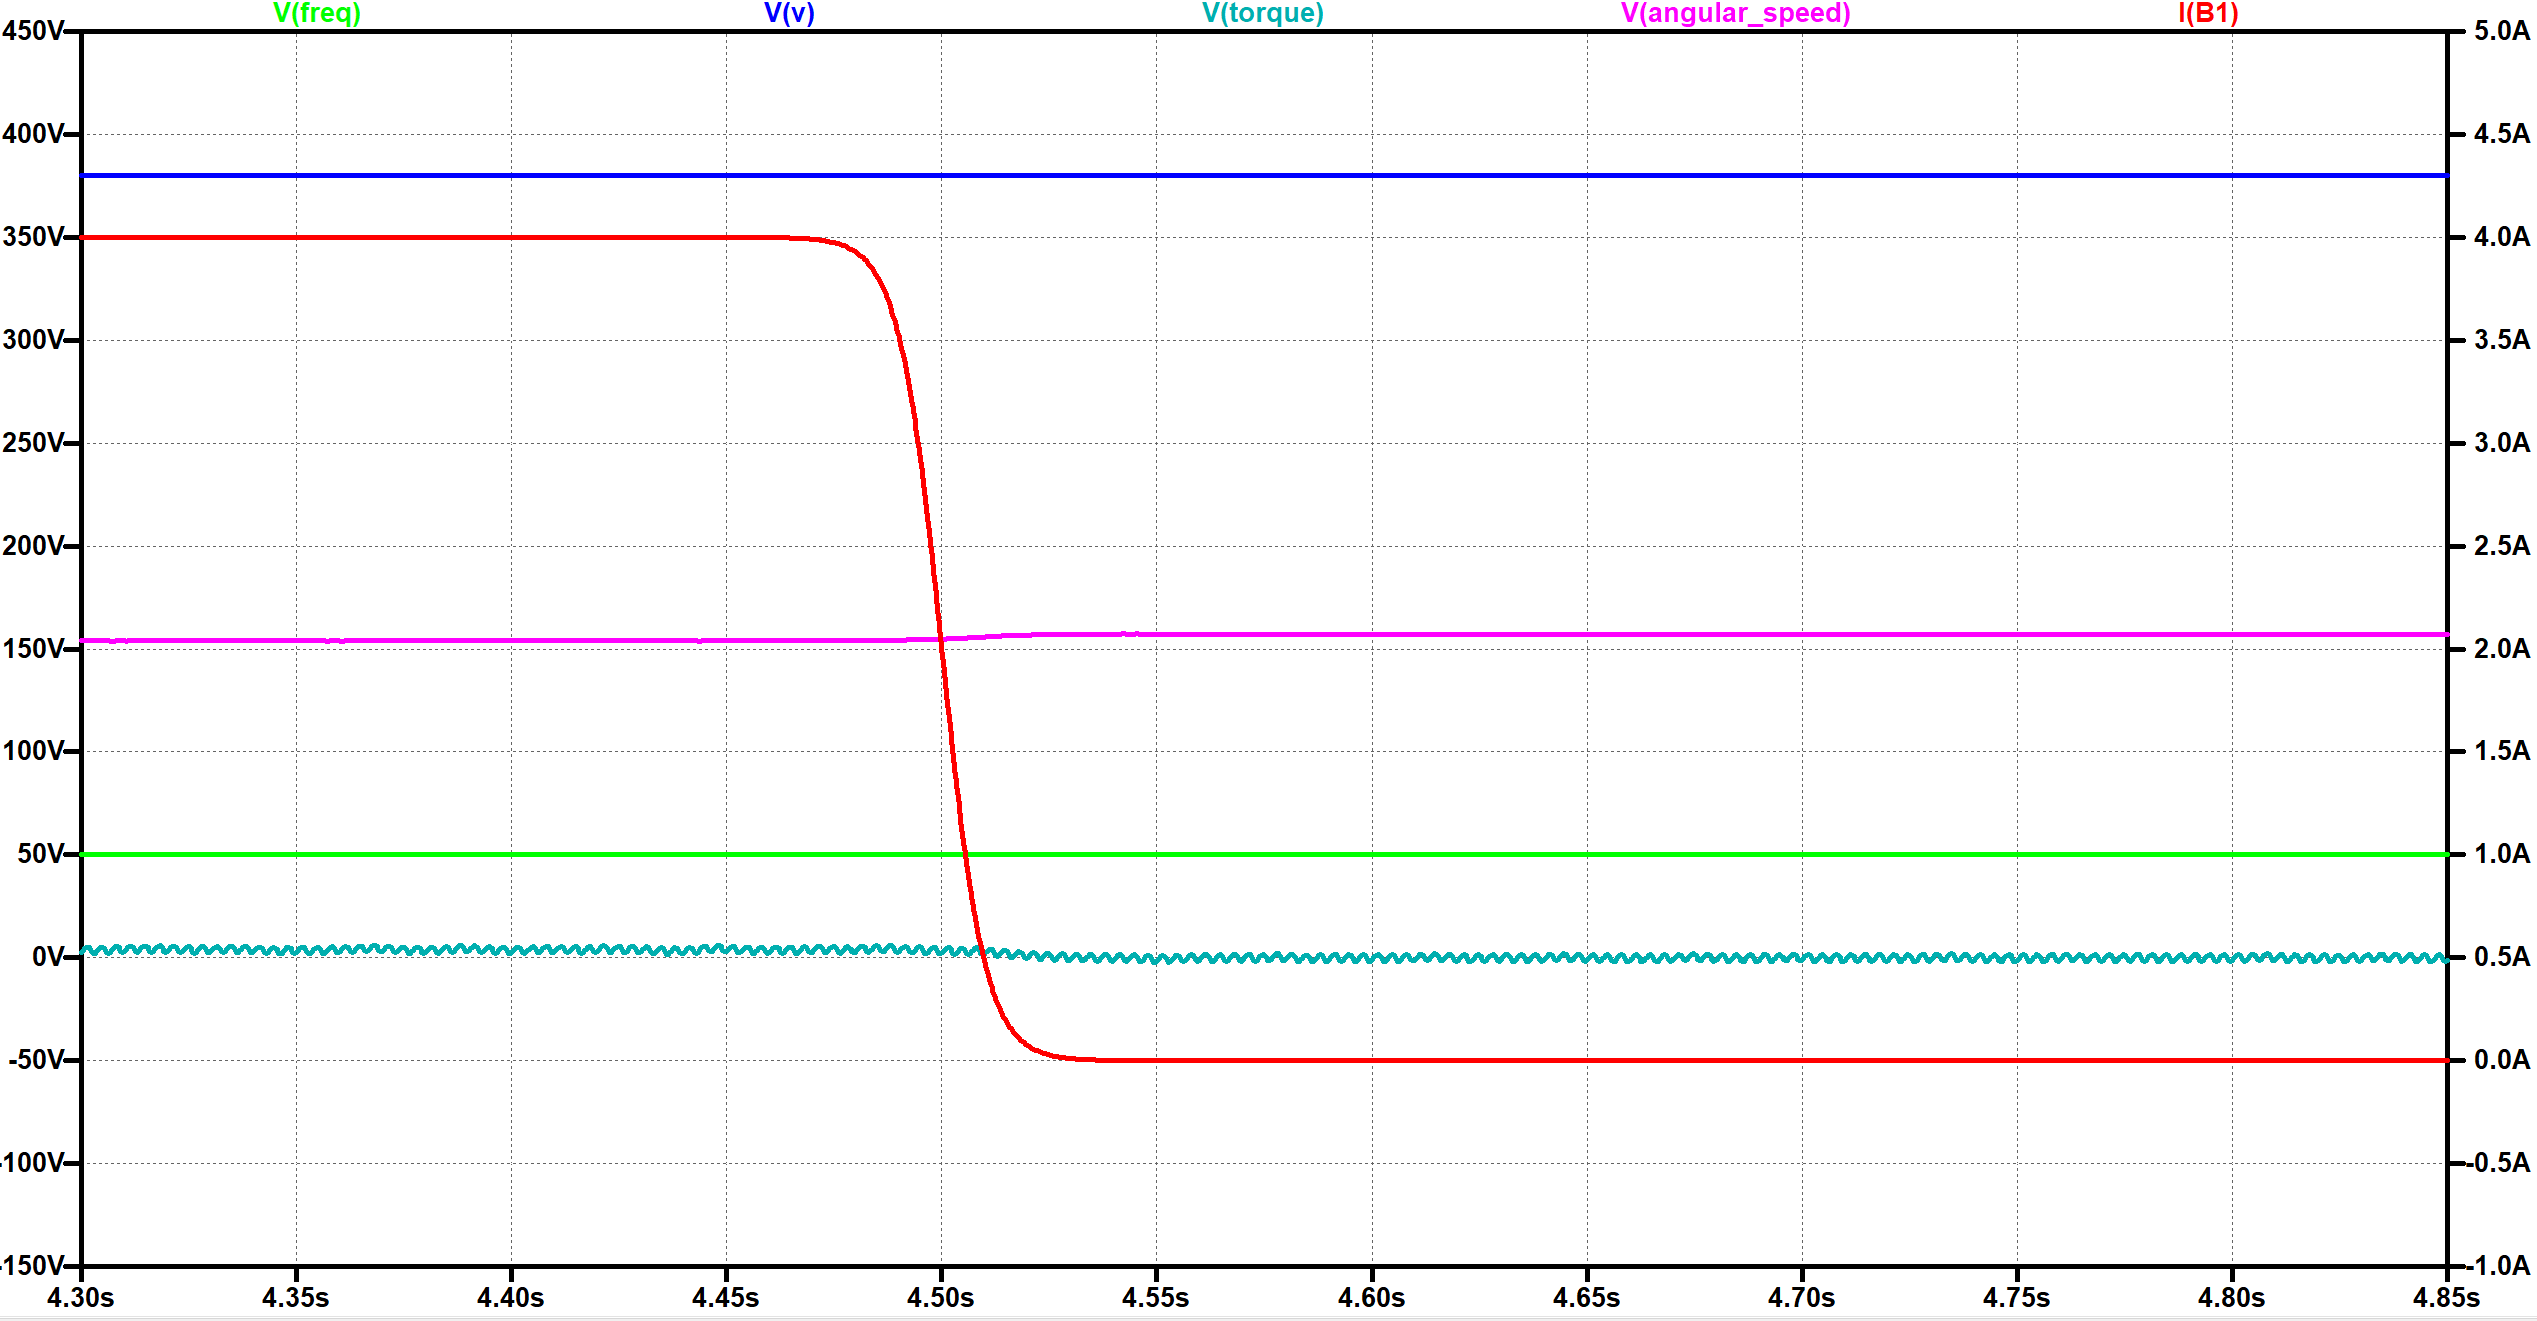
\includegraphics[width=0.45\linewidth]{Imagenes/3-1-a-descarga.png}
\caption{Simulación de la carga y descarga al motor}
\end{figure}

Cuando cargamos al motor en el momento en que I(B) sube, lo que ocurre es que el motor sufre una merma en su velocidad, es decir frena; y a su vez el torque aumenta hasta que ambos valores se estabilizan nuevamente. Estas variaciones se arrojaron valores de $\Delta V_{angular_speed}=3.12 V$ y $\Delta V_{torque}=1.795 V$.
Cuando la carga es liberada (es decir se deja de drenar corriente), ocurre el efecto opuesto, disminuyendo el torque a 0 y aumentando la velocidad angular a la original.
\subsubsection{Interpretación de Variables físicas del Spice}
Si bien las variables mencionadas anteriormente fueron obtenidas en tensiones debido a que así es como están modeladas en Spice, lo que ocurre es que esos valores de tensión representan unidades del SI. A continuación indicamos cuáles son esas unidades a las que representan:

\begin{table}[H]
\centering
\begin{tabular}{@{}ccc@{}}

Variable medida   & Unidad Representada     & Relación unidad/V \\ \midrule
Frecuencia        & Hz                      & 1                 \\
Torque            & $kg \cdot m^2$ & 1                 \\
Velocidad Angular & RPM                     & 60                \\
Carga (Torque)    & $kg \cdot m^2$ & 1                 \\ \bottomrule
\end{tabular}
\caption{Tabla de interpretación de las unidades tomadas del LTSpice}
\end{table}

\end{document}